\documentclass[UTF8,9pt]{report}
\usepackage{CTEX}
\usepackage{../template/Notes/notes}
\usepackage[colorlinks,linkcolor=red]{hyperref}
\title{11组-8题报告-Slinky 弹簧} 
\author{肖涵薄,高晗,王杏之,王子毓,郑雯文}
\begin{document}
\maketitle
\tableofcontents

\chapter{题目概述} 
\se{Slinky弹簧介绍}
\begin{center}
    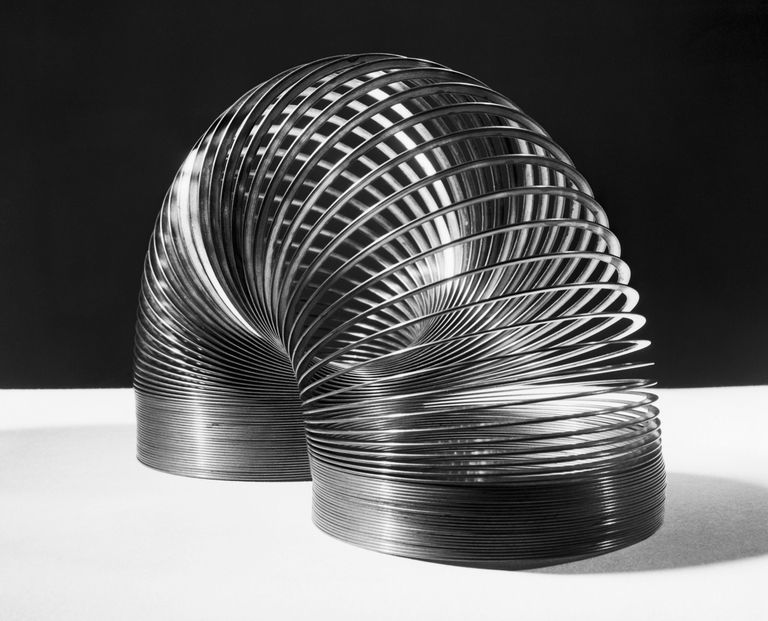
\includegraphics[scale=0.2]{1536562195277425.jpg}
\end{center}
我们研究上图这样一个弹簧,它有一个特殊的名称--- ``Slinky弹簧"。
\begin{center}
    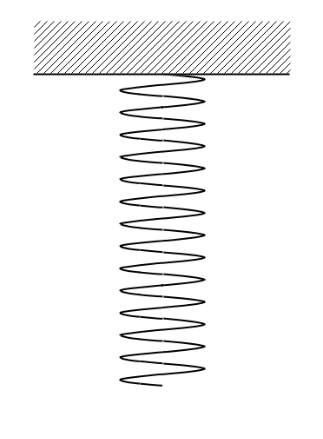
\includegraphics[scale=0.7]{1_1.png}
    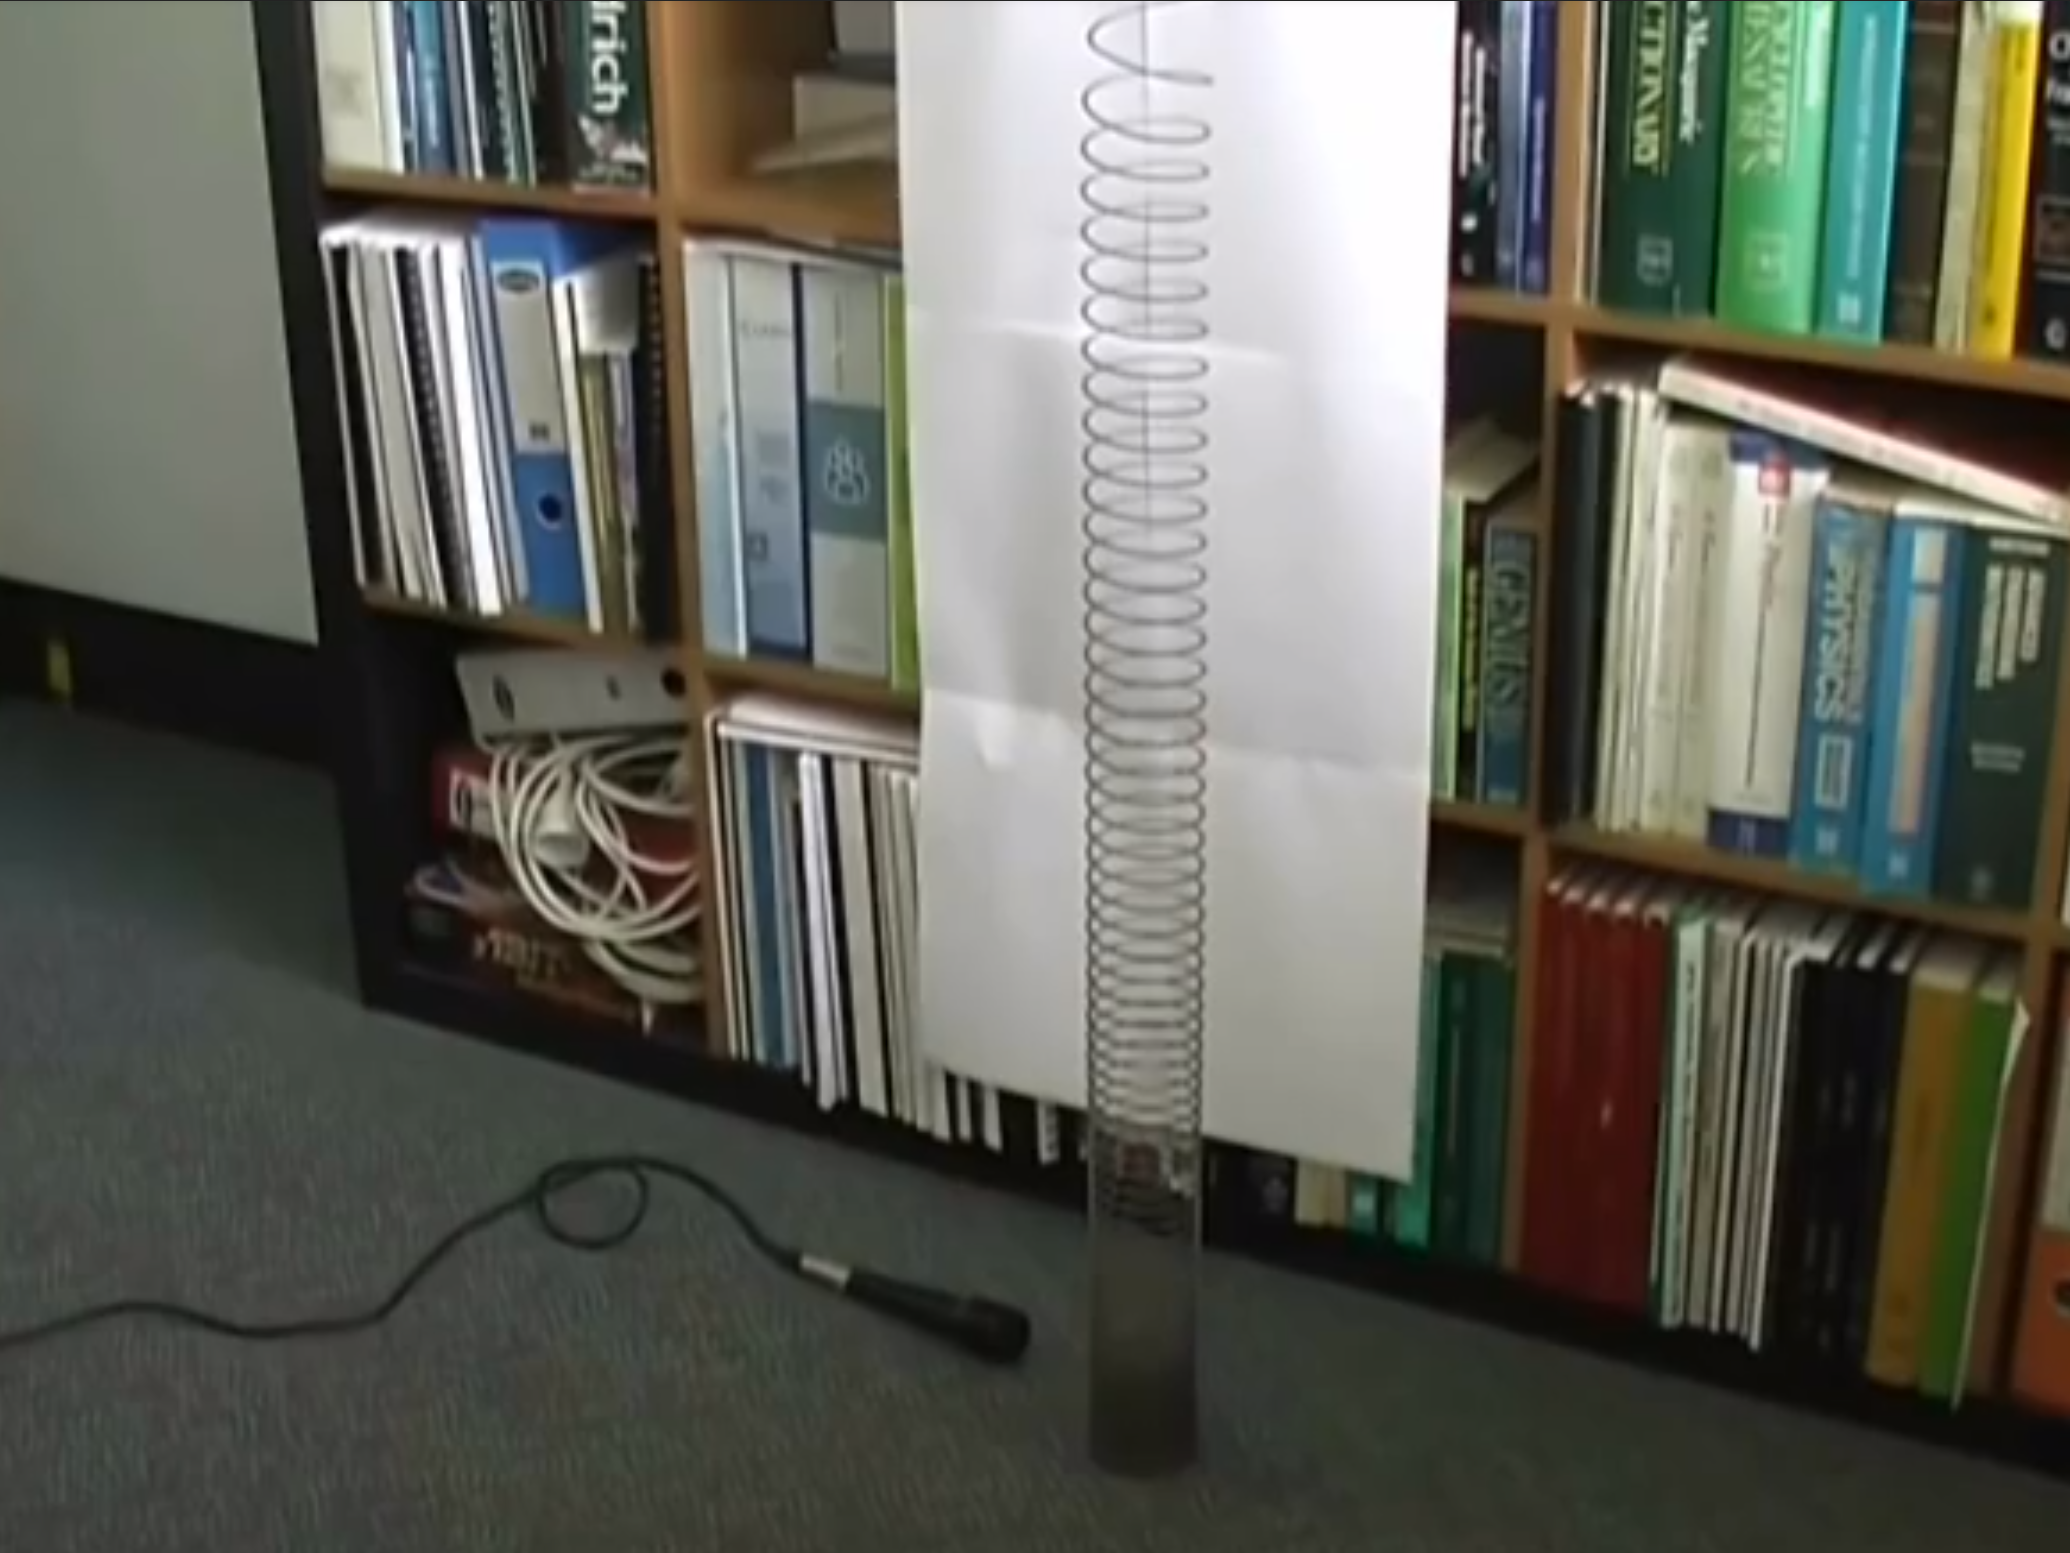
\includegraphics[scale=0.2]{1_12.png}
\end{center}
当我们把弹簧像上图这样一端悬挂固定(约2-3m),并敲击螺旋弹簧,可以模拟出类似科幻电影中“激光枪”的声音。我们希望能解释这一现象。
\subsection*{该弹簧具有如下的性质:}
弹簧具有质量分布:
    $$p(n)=L(n-1)^2$$
    其中$n=\text{该点上方质量/总质量}  $, $n \in [0,1]$,$p(n)$给出了$n$以slinky底部为原点向上的位置。\\
波速与激波:由于弹簧太软只能拉伸不能压缩, 弹簧自由塌缩的速度快于弹性波波速时( 自由塌缩指的是始终满足胡克定律的弹簧自由振动塌缩的速度 ), 会出现波源运动速度比波速快的现象, 因此弹簧中会出现冲击波(激波). 而冲击波传播到末端的时间要比自由弹性波短很多.\\
高柔软度:\\
    其轴向刚度k=0.003N/mm(compared with 1-200N/mm for others)\\
    动图:\url{https://pic2.zhimg.com/v2-f46e972de8f2df71ab6753e39a60b819_b.gif}
    \putfig{0.7}{1_17.png}
\se{我们要寻找的声音}
    \putfig{1}{1_22.png}
    对视频资料中的实验进行简单分析,上图即为所谓的科幻电影中“激光枪”的声音,上方为其波形图,下方纵轴为频率,对某一频率比例越大颜色越黄,其振幅较大的一段持续时间约为$12ms$.\\
    下图左方为$1.2ms$处频谱图,右方为$10ms$处频谱图。可以观察到,其频率随时间单调递减,振动初始时间频率大约为$9kHz$,$10ms$前后频率降至$500Hz$\\
    \begin{center}
        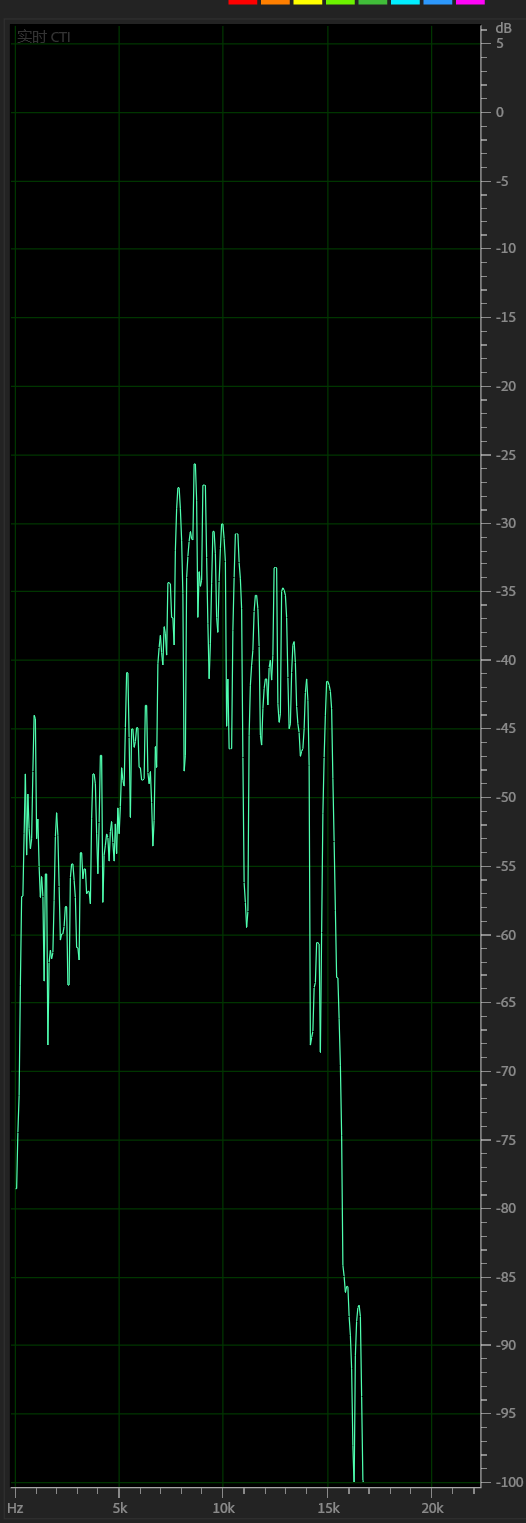
\includegraphics[scale=0.4]{1_20.png}
        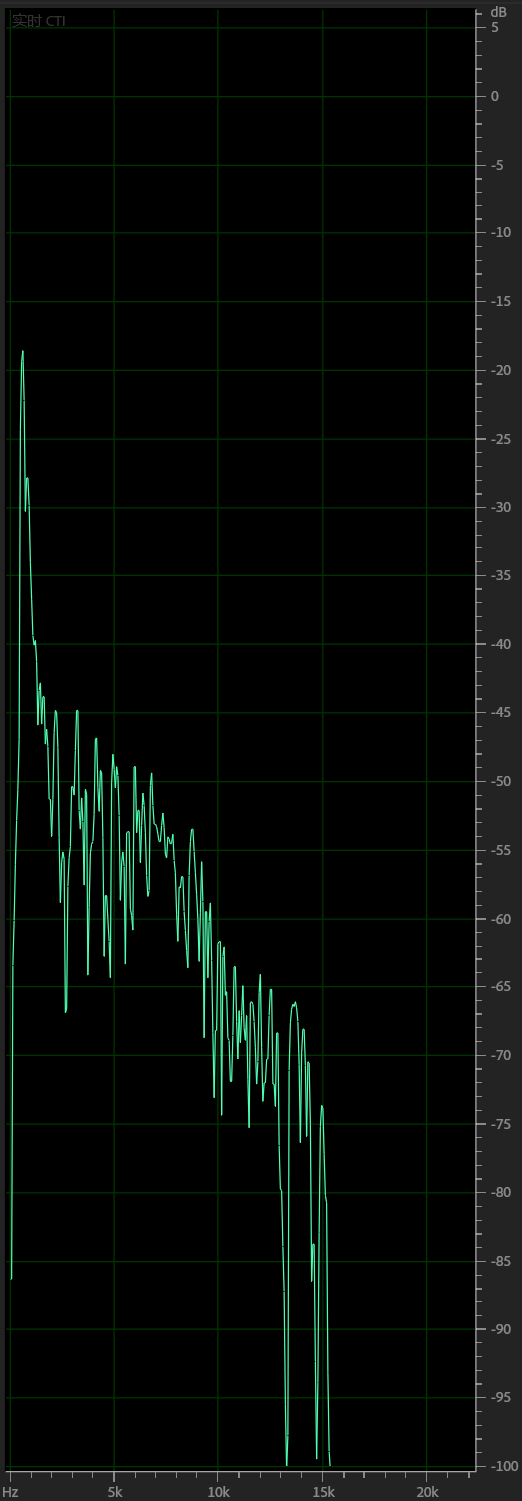
\includegraphics[scale=0.4]{1_21.png}
    \end{center}
    频率降低的原因:Slinky和一些与之类似的弹簧可用于制造类似“激光枪”音效。把Slinky搁置在空中,轻敲一端,便可以在另一端接受到骤然降低的金属音效。这是因为在金属中,高频声音的传递比低频更快{\color{red}(为什么高频波更快?)},所以在接收端先听到的是的尖啸的高音,然后才逐渐降低。--百度百科\url{https://baike.baidu.com/item/Slinky} \\
    我们希望能在实验中复现这个逐渐降低的频率,并得到更清晰的图像,与此同时,我们会把弹簧的每个宏观状态与波的每个传播阶段做对应。
\se{目标与变量}
    我们希望定量的得到弹簧振动的频率分布,波速,以及弹簧自身形状(长度,横截面积,弹性模量等)如何影响这个波,阻尼如何影响各个频率的波,并将理论与实验比较。进一步地,希望能通过理论模型得到之前没有考虑到的影响因素,或预测一些现象,并在实验中验证它。
\chapter{理论部分}
\se{EULER-BERNOULLI梁理论}
若将如图弹簧拉直(受重力后略向下垂),并认为拉直后弹簧振动模式不会发生变化,则可使用梁理论对弹簧的振动模式进行分析。\\
\putfig{0.4}{1_0.png}
同时还要进行如下假设:\\
(1) 光束是棱柱形的,有一个直的质心轴,我们把它标为x轴。\\
(2) 梁的截面有一个对称轴,将其标记y轴。\\
(3) 所有横向荷载均作用于对称平面(x - y平面)。\\
(4) 垂直于质心轴的平面截面在平面变形后始终保持不变。\\
(5) 材料为弹性材料、且为各向同性、均质的。\\
(6) 横向挠度小。\\
(7) 运动在y方向上是纯平动的,即转动效应可以忽略,这个假设将在后文Rayleigh梁理论和Timoshenko梁理论中移除。\\
(8) 梁单元在运动过程中保持矩形,这个假设将在后文Timoshenko梁理论中移除。\\
取弹簧的一个微元如下图所示,M代表弹簧内禀的弯矩,V代表弹簧内禀的剪力,w代表外部施加的负载,在该问题中即为弹簧自重。\\
\putfig{0.7}{1.png}
类比牛顿第二定律,有如下关系(其中$\rho$为密度,A为横截面积):
\begin{equation}\frac { \partial V } { \partial x } = - w + \rho A \frac { \partial ^ { 2 } y } { \partial t ^ { 2 } } \label{5.1}
\end{equation}
且(证明:\url{http://kjwy.5any.com/jzlx/content/jzlx05/jzlx-kcjj-050501.htm})
\begin{equation}
    \pp{M}{x}=V \label{5.2}
\end{equation}
由上面两式可得到:
$$\frac { \partial ^ { 2 } M } { \partial x ^ { 2 } } = - w + \rho A \frac { \partial ^ { 2 } y } { \partial t ^ { 2 } }$$
再代入胡克定律$\sigma=E\epsilon$(需要假设(4-6),其中E为弹性模量,I为z轴的截面惯性矩(截面二次轴矩)).
\begin{equation}
\frac { \partial ^ { 2 } y } { \partial x ^ { 2 } } =-\frac { M } { E I} \label{5.4}
\end{equation}
将其代入后则可得到Euler-Bernoulli beam理论方程:
\begin{equation}
    EI\pp[4]{y}{x}+\rho A\pp[2]{y}{t}=w \label{5.5}
\end{equation}
若不考虑重力,即$w=0$。可化为齐次方程:  {\color{red}考虑到弹簧比较轻,可能可以不考虑重力,我们后期会对比考虑重力与不考虑重力的解差距是否大,该近似是否可行。}
\begin{equation}
    b^2\pp[4]{y}{x}+\pp[2]{y}{t}=0,\quad b^2=EI/\rho A \label{5.6}
\end{equation}
\se{分离变量法得到半定量模型}
假设$y(x,t)=X(x)T(t)$,代入\ref{5.6},可以得到2个分离的解:
$$\begin{array} { l } { x ^ { \prime \prime \prime \prime } - \frac { \gamma ^ { 2 } } { b ^ { 2 } } x = 0 } \\ { \ddot { T } + \gamma ^ { 2 } T = 0 } \end{array}$$
其中$\gamma$为分离常数,上面这个两方程的通解为:
$$X (x ) =C _ { 1 } \sin \sqrt { \frac { \gamma } {b } }x +C_ { 2 } \cos \sqrt { \frac { \gamma } {b } }x+ C _ { 3 } \sinh \sqrt { \frac { \gamma } {b } }x +C _ { 4 } \cosh \sqrt { \frac { \gamma } {b } }x$$
$$T ( t ) =C _ { 5 }  \sin\gamma t +C_ { 6 }$$
假设弹簧的顶部和底部均固定,则没有挠度和弯矩,此时有边界条件
$$y(0)=\ddot{y}(0)=0$$
$$y(l)=\ddot{y}(l)=0$$
代入微分方程\ref{5.6},得到:
$$C_2=C_4=0$$
$$\ip \begin{array}{rl}
    C _ { 1 } \sin \sqrt { \frac { \gamma } {b} } l +C _ { 3 } \sinh \sqrt { \frac { \gamma} { b } } l &= 0\\
- C_ { 1 } \sin \sqrt { \frac { \gamma } {b}} l +C _ { 3 } \sinh \sqrt { \frac {\gamma } {b } } l &= 0
\end{array}$$
上式唯一的非零解为:
$$\sqrt{\f{\gamma}{b}}l=n\pi,\quad for\ n=0,1,2...$$
$$\ip \gamma _ {n} = \frac {n^ { 2 } \pi ^ { 2 } } { l ^ { 2 } } b= \frac {n^ { 2 } \pi ^ { 2 } } { l^ { 2 } } \sqrt { \frac { EI} { \rho A} }$$
这个波具有无穷多个离散的频率,其解为:
$$y ( x , t ) = \sum _ { n = 1 } ^ { \infty } \sin \frac { n \pi x } { l } ( A_ { n } \sin \gamma _ { n } t +B_ { n } \cos \gamma _ { n } t )$$
下图为一篇文献中对该弹簧振动的频谱图,可见其频率的确是离散的:\\
\url{http://research.spa.aalto.fi/publications/papers/dafx10-slinky/}
\putfig{1}{1_26.png}

\se{RAYLEIGH梁理论}
基本的欧拉-伯努利束理论对于高频运动有一些严重的缺陷。为了解释梁单元的旋转运动,我们对这一理论作了进一步的改进,此时梁单元的角加速度将被纳入分析中,$\ref{5.2}$式变为:{\color{red} 为什么?}
\begin{equation}
    \frac { \partial M } { \partial x } = V - \rho I \frac { \partial ^ { 2 } \theta } { \partial t ^ { 2 } } \label{5.34}
\end{equation}
其中$\t$为转动角度。
对于小的变形,近似$\t \approx \pp{y}{x}$,上式变为:
$$\frac { \partial M } { \partial x } = V - \rho I \frac { \partial ^ { 3 } y } { \partial t ^ { 2 } \partial x }$$
联立\ref{5.1},\ref{5.4},a
可化简得到:
\begin{equation}
    b ^ { 2 } \frac { \partial ^ { 4 } y } { \partial x ^ { 4 } } - a ^ { 2 } \frac { \partial ^ { 4 } y } { \partial x ^ { 2 } \partial t ^ { 2 } } + \frac { \partial ^ { 2 } y } { \partial t ^ { 2 } } = 0,\quad b^2=\f{EI}{\rho A} ,a^2=\f{I}{A} \label{5.36}
\end{equation}
此即Rayleigh梁理论方程。
\se{TIMOSHENKO梁理论}
上一节修正了基本的Euler-Bernoulli定理来解释旋转运动。现在我们进一步完善理论,以考虑剪切变形。Timoshenko在发展这一理论时已经证明,对于高频振动,剪切变形至少与旋转惯性同样重要。因此现在我们将修正$(2)$,保留旋转和剪切效应。\\
我们将注意力转向剪切变形情况。在这种情况下,梁微元的横截面不再垂直于x轴或侧方。\\
这种情况如下图所示,其中$\psi$表示横截面与y轴夹角,横截面的剪切应变此时为$\pp{y}{x}-\psi$
\putfig{0.7}{1_5.png}
此时$M,V$变为:{\color{red} 为什么?}
$$\begin{array} { l } { M = - E I \frac { \partial \psi } { \partial x } } \\ { V = k ^ { \prime } \mu A \quad ( \frac { \partial y } { \partial x } - \psi ) } \end{array}$$
其中$\mu$为剪切模量,$k'$为取决于横截面形状的剪切常数  {\color{red}这是多少?怎么测?}.\\
将上面两式代入,前面的\ref{5.34}式现在变为:
$$EI\frac { \partial ^ { 2 } \psi } { \partial x ^ { 2 } } + k ^ { \prime } \mu A \quad ( \frac { \partial y } { \partial x } - \psi ) - \rho I \frac { \partial ^ { 2 } \psi } { \partial t ^ { 2 } } = 0$$
还是代入这两个式子,对于$w=0$的情况,前面的\ref{5.1}式现在变为:
$$k ^ { \prime } \mu ( \frac { \partial ^ { 2 } y } { \partial x ^ { 2 } } - \frac { \partial \psi } { \partial x } ) - \rho \frac { \partial ^ { 2 } y } { \partial t^ { 2 } } = 0$$
通过这两个式子消去$\psi$:
\begin{equation}
    b ^ { 2 } \frac { \partial ^ { 4 } y } { \partial x ^ { 4 } } + \frac { \partial ^ { 2 } y } { \partial t ^ { 2 } } - a ^ { 2 }( 1 + \frac { b ^ { 2 } d ^ { 2 } } { a ^ { 2 } }) \frac { \partial ^ { 4 } y } { \partial t ^ { 2 } \partial x ^ { 2 } } + a ^ { 2 } d ^ { 2 } \frac { \partial ^ { 4 } y } { \partial t ^ { 4 } } = 0 ,\qquad  b^2=\f{EI}{\rho A} ,a^2=\f{I}{A}, d^2=\f{\rho}{k'\mu} \label{5.47}
\end{equation}
式\ref{5.47}为Timoshenko梁理论方程,包括旋转校正和剪切校正。注意在这个表达式中,前两项对应于初等情况;第三项包含转动惯量瑞利校正项和剪切校正项;最后一个量是旋转校正和剪切校正之间的耦合项。
\se{采用Timoshenko梁理论求解方程}
考虑沿x轴无限延伸的梁的自由振动。假设梁从静止状态以零速度从规定位置$f(x)$释放。此时的边值问题为:求解\ref{5.6}式当具有初始条件
$$y(x,0)=f(x)$$
$$\dot{y}(x,0)=0$$
显然,任意形式的波型$f(x + ct)$或$g(x - ct)$不满足欧拉-伯努利梁方程(\ref{5.6})。因此,扰动不能以相同的速度传播,波形必须发生色散,见下图。它比较了梁运动(实线)和柔性弦运动(虚线)。通过选择常数b,使梁的平均波速近似等于弦运动的相速度。与柔性弦的非色散运动相比,该图清楚地展示了梁运动的色散特性。{\color{red}柔性弦如何运动?}
\putfig{0.7}{1_7.png}
为了进一步研究这种色散现象,让我们尝试简谐波解,
$$y(x,t)=A\cos[k(x \pm ct)]$$
将简谐波代入\ref{5.47}式:
$$c ^ { 4 } - \frac { 1 } { a ^ { 2 } d ^ { 2 } } ( a ^ { 2 } + b ^ { 2 } d ^ { 2 } + \frac { 1 } { k ^ { 2 } }) c ^ { 2 } + \frac { b ^ { 2 } } { a ^ { 2 } d ^ { 2 } } = 0$$
上式虽然有四个根,但只有两个具有物理意义{\color{red} 为什么?是因为另外两个为虚数吗?}。这两个根通常给出一个相速度依赖关系,如下图所示。
\putfig{0.7}{1_9.png}
群速度关系{\color{red} 怎么求?}如图,群速度与相速度极限相同:
\putfig{0.7}{1_10.png}

\se{查阅到的另外几种可建立理论模型的方法}
以下几种方法均来自Reference-kit:\url{http://stemfellowship.org/wp-content/uploads/2016/11/iypt-kit-2019.pdf}
\sub{有限差分}
有限差分可以对微分方程离散化,进行离散逼近。
\subsection*{波导}
\subsection*{螺旋运动矩阵}
\subsection*{驻波}
推导声波纵波与弹簧谐波关系-利用驻波。
\chapter{实验部分}
\se{设计实验时的思考}
\sub{如何产生振动?}
    根据网上查阅到的资料,产生振动大多为两种方法:\\
    1. 用手竖直方向拨动弹簧,拿开手后弹簧即产生声音,但噪声较大.\\
    2.将弹簧底部拿起约0.3m,放开手任弹簧底部落下,同样产生声音,这个方法噪声较小,但视频中弹簧落到地上的一瞬间会产生巨大的噪声,由于弹簧落地的一瞬间也是刚开始产生我们所需要的声音的一瞬间,因此我们希望能消除这段噪音。{\color{red}那么是不是可以将弹簧离地远一些,使其落下时不会接触地面呢?弹簧如果没有落地还会产生我们所需要的声音吗?在哪种情况下现象最明显?}\\
    我们对振源的要求是:\\
    1. 能产生足够幅度的振动\\
    2. 可以产生简谐振动,简谐振动不仅计算更简单,且解出简谐解后通过线性叠加可以得到任意波的解。\\
    3. 可以产生较宽的频域,这样就能测量不同频率的振源对弹簧的影响了。\\
    4. 价格较低,或实验室已有。\\
    在与多位实验老师沟通后,我们最终选择直接用大功率音响做波源,同时我们也会测量上面两种方法产生的波并试图解释。
\sub{如何收集振动?}
    在查阅一些文献后,我们发现不同频率的波在弹簧中会产生色散,因此除了弹簧内波的频率,其传播速度也是一个值得探讨的问题。为了同时能测出弹簧内部波的频率和波速,我们需要能同时测量频域和时域的探测器。同样,由于弹簧内部存在频率差距较大的波,测量仪器要对较宽频域的波都有灵敏的响应。\\
    在与多位实验老师沟通后,我们最终选择适用于近场拾音的心形指向电容麦克风收集弹簧振动产生的声音。我们猜测,波源停止振动后,两次测到同一频率的波的时间差即为该频率的波在弹簧中传播一个来回的时间。\label{time}
\sub{如何处理数据?}
    由于麦克风输出的是模拟信号,我们拟将麦克风输出端连接至示波器,记录数据并导出至电脑处理,不直接用电脑录音的原因是我们猜测电脑模电转换模块的性能不如示波器,若实际实验时发现二者相近,则可直接将麦克风连至电脑录音。
\se{实验步骤}
\putfig{0.5}{1_11.png}
实验仪器如图所示,实验主体为弹簧,起振器发出简谐波,引起弹簧振动,麦克风采集弹簧振动产生的声波。\\
\sub{STEP 0:观察振动}
    先引发一个明显的波,通过摄像机记录,观察波在弹簧里如何传播,波速如何,有无色散,持续时间为多久?\\
在实际实验中,我们可能会对实验仪器和仪器的位置进行多次调整。
\sub{STEP 1:测量标准弹簧}
    首先测量一个定为标准的弹簧的各个参数,括号外为公式中体现的物理量,括号内为直接测量的物理量:弹簧长度(匝数,直径),截面积(粗细),杨氏模量(劲度系数),其他影响材质的量(未定)
\sub{STEP 2:调整起振器}
    改变起振的振幅及频率:观察起振器不同的振幅和频率如何影响实验现象\\
    改变起振方向:把纵波变为横波,观察是否还有相同现象。\\
    改变起振位置:在上图中我们将起振器放置在了弹簧顶端。此时外力的波的边界条件在$x=0$处,作用效果为一个由上至下传播的波。当我们把起振器插入弹簧中间某一段起振,我们猜测:由于弹簧长度较长,远远大于波长(波长=周期$\times$波速,波速很小)(这个猜测需要后续实验验证),可以将其视作无限长弹簧,则理论分析中的边界条件可用与该情况。
\sub{STEP 3:调整弹簧}
    我们预计采购匝数(对应理论中弹簧长度)不同的弹簧,测量不同弹簧内部波传导的方式有何不同,并与理论比较。由于厂家限制,无法定制杨氏模量不同的弹簧,我们可能在后面通过其他方法测出弹性模量如何影响波的传导。
\sub{STEP 4:调整麦克风}
    在上图中麦克风固定在桌面,位于弹簧侧面,除了这种放置方法我们还有两种方法:
    1. 置于弹簧底部, 这样我们可以测出同一个频率的波两次到达弹簧底部的时间差,根据\ref{time}处最后一句话的假设,我们可以测出不同频率波速。
    2. 固连在弹簧上,这样可以收集到不易在空气中传播的低频波,但由于麦克风随弹簧振动,会对弹簧振动产生干扰,且会产生较大的噪音。
\se{一个文献中的实验}
以下方法来自Reference-kit:\url{http://stemfellowship.org/wp-content/uploads/2016/11/iypt-kit-2019.pdf}
使用压电换能器,测量脉冲响应实验显示,其色散为低频比高频传播慢。\\
\url{http://dafx10.iem.at/papers/ParkerPenttinenBilbaoAbel_DAFx10_P80.pdf}\\
使用无量纲形式伯努利方程:
$$\frac { \partial ^ { 2 } u } { \partial t ^ { 2 } } = - \kappa ^ { 2 } \frac { \partial ^ { 4 } u } { \partial x^{4}} + \left[-2\sigma _0\frac { \partial u } { \partial t } + 2 \sigma _ { 1 } \frac { \partial ^ { 3 } u } { \partial t \partial x ^ { 2 } } \right]$$
其中$u$为横向位移,$x$为沿弹簧轴方向的位置,$t$为时间,$\kappa$为与密度,杨氏模量,长度有关的无量纲常数(需要用实验确定大小)。括号内为对理想杆的修正,$\sigma$控制损失特征[S. Bilbao,Numerical Sound Synthesis, John Wiley and Sons,2009]\\
现假设脉冲从$x=0$传导至$x=1$,考虑理想杆模型$(\sigma_0=\sigma_1=0)$,有特定频率
$$T _ { D } = \frac { 1 } { 2 \sqrt { 2 \pi \kappa f } }$$
表达式给出了色散下第一个到达的波,通过该式可求得$\kappa$(求出后与实验对照)。\\
其中需要通过FIR带通滤波测量频率,且两次测到该频率的时间间隔给出该波传播花费的时间。
\begin{comment}
\chapter{参考文献}
\begin{itemize}
\item \url{https://en.wikipedia.org/wiki/Slinky}
\item \url{https://en.wikipedia.org/wiki/Euler%E2%80%93Bernoulli_beam_theory}
\item Parker, Julian, et al. "Modeling methods for the highly dispersive slinky spring: a novel musical toy." Proceedings of the 13th International Conference on DigitalAudio Effects (DAFx’10). 2010.\\
\url{http://dafx10.iem.at/papers/ParkerPenttinenBilbaoAbel_DAFx10_P80.pdf}
\item Lee, J., and D. J. Thompson. "Dynamic stiffness formulation, free vibration and wave motion of helical springs." Journal of Sound and Vibration 239.2 (2001): 297-320. \\
\url{https://www.sciencedirect.com/science/article/pii/S0022460X00931699}
\item Rutherford, Casey. "A Fresh Look at Longitudinal Standing Waves on a Spring." The Physics Teacher 51.1 (2013): 22-24.\\
\url{https://www.researchgate.net/profile/Casey_Rutherford/publication/258810726_A_Fresh_Look_at_Longitudinal_Standing_Waves_on_a_Spring/links/5695160e08ae820ff0749c0f.pdf}
\item \url{https://www.researchgate.net/post/Why_does_tapping_in_air_not_produce_any_sound_but_tapping_against_a_metal_does_produce_sound}
\item \url{https://www.youtube.com/watch?v=g2Sa0dRmHgA}
\item \url{https://www.youtube.com/watch?v=CpZkNWBmKNM}
\item \url{https://www.youtube.com/watch?v=7VGlBZOywIg}
\item \url{https://www.youtube.com/watch?v=aqtqiuSMJqM}
\item \url{https://www.youtube.com/watch?v=rajPbk3CJr4}
\item \url{https://www.youtube.com/watch?v=SVAd6zxjiow}
\item \url{https://www.youtube.com/watch?v=XACHZbgcH5M}
\end{itemize}
\end{comment}
\end{document}